\documentclass[12pt,]{article}
\usepackage[T1]{fontenc}
\usepackage[utf8]{inputenc}
\usepackage{fullpage}

% \usepackage{authblk}
\usepackage{graphicx}
\usepackage{import} 
\usepackage{subfig}
\graphicspath{{../../results/}}

\usepackage[left]{lineno}
\linenumbers

\usepackage{todonotes}

\title{A comprehensive study of the early phylodynamics of SARS-CoV-2 in Europe}

\begin{document}
\maketitle

\abstract{This project focus on the spatial dynamics of the early spread of SARS-CoV-2 in Europe. We apply a novel approach based on the Multi-type Birth Death phylodynamic model to infer structured population dynamics jointly with between-subpopulation transmission rates from viral genome sequences. The inferred epidemic trajectories for the combined outbreak responsible for the observed sequence data will allow us to better understand the entry into and early spread of SARS-CoV-2 in Europe.}

\section*{Introduction}

\section*{Methods}

\section*{Results}

\subsubsection*{Total case counts}

Figures \ref{fig:gribbon} and \ref{fig:trajs}.\\

Inferred population trajectories that account for all cases in the country. It is not an independent estimate since we are using informative priors for the sampling rates (upperbound computed as sequences/reported cases) and the subsampling scheme also includes the number of cases in the country (but that is a weaker link I think.\\

Comparison with ECDC case counts: delay in notifications and underreporting, for some of the  countries at the end of the periord the reported cases are very closed to the trajectories, e.g. Italy, Germany. Hubei-China huge difference in tendency and absolute numbers.\\ \todo{Working on these with new analyses}

Measure the (mean?) difference between inferred and reported case counts and compare among countries. By day or in general? Absolute or relative to the number of cases that day?

\subsubsection*{First introductions}
Figures \ref{fig:first}, \ref{fig:first_src} and \ref{fig:first_dest}.\\

We want to answer the question of when and where the first case in Europe occured. No clear, Germany? Figure \ref{fig:first} A. We can measure the time between first case and first reported case and compare between countries. \\
\todo{ticks for every month}
And for each country where this first case came from, more support for Hubei introduction in all countries Figure \ref{fig:first} B.\\

Measure expected day of introduction.

In Figure \ref{fig:first_src}, we are looking at the ordered set of introduction intoo european countries. For each trajectory, we have the fist introduction into each country happening in a determined order, i.e. the first european country with a covid case, the second country with a covid case... So we are vissualizing the number of trajectories that share the same order of first cases. More trajectories where the first case was to Germany, no clear order after the first country. Spain last one.\\
\todo{Explain this better}

In Figure \ref{fig:first_dest} we are looking at the ordered set of countries spreading covid. In the first position we have Hubei for all trajectories since it is the origin of the epidemic. In second position we will have the first European country from where a covid case was imported to other country. No clear dynamics except that moore support for Spain being the last country having a first exported covid case. Germany first one.\\  

\subsubsection*{Migration vs within-region transmission}

Figure \ref{fig:events}\\.

This question is addresed on the original paper from Sarah.  Maybe could be interesting to look at this perspective since it is important for border closure measures.

\todo{Think about results}
 Not sure if we can have any meaningful results insights on the topic. Migrations started very early in our analysis to all european countries. Withing regions transmision account for most of the cases in the countries from late january onwards (when first cases were being reported in Europe).\\

 Measure the time between the first outcoming mirgration from the country  (specially interesting for Hubei) and first reported case. This could be interesting to say if a extreme measure closing borders with the first case could be effective to impede transmission to other countries: percentage of trajectories whre transmission to Europe would have been avoided. For other countries we can look at how many migrations events could have been avoided (and how many not) if the country closed borders after first reported case.\\ 

 Measure the time between first birth/migration and first reported case and compare between countries. How well did the countries detecting the first cases, there were already within region transmision?\\

 Measure the time between the first migration into a country and the first birth in the country. Or the first outcoming mirgration from the country and first birth. This could be interesting to say if we should focus or not the screening and testing capacities to detect incoming migrations or a more general strategy to find cases in the population. Is it different for each country?\\


\subsubsection*{Migrations patterns}
Figures \ref{fig:migs_srcdest} and \ref{fig:migs}.\\

Similar information in both plots, but in the chord plots instead of a dayly evolution the time period is split on three (as in the GLM analysis). Chord plots are nicer and easier to understand I think, but barplots shows the great detail of the results of the model. Another advantage of the chrod plot is that the ir shows mean absolute values and not only relative values.\\

Hubei-China is the majority source of migrations for all countries till February and then some patterns emerge (we expect more interesting results with the added info in GLM analysis).\\


\todo{Legend in plot 7 and change white text}

\subsubsection*{GLM predictors}
Which channels were the main sources of transmission across national borders.

\subsubsection*{Epidemiological parameters}

Not sure about this section. But maybe it make sense for completeness to include, briefly, the values of estimate R0, migration and sampling rates.


\section*{Discussion}

\section*{Conclusion}


\begin{figure}[ht]
    \centering
    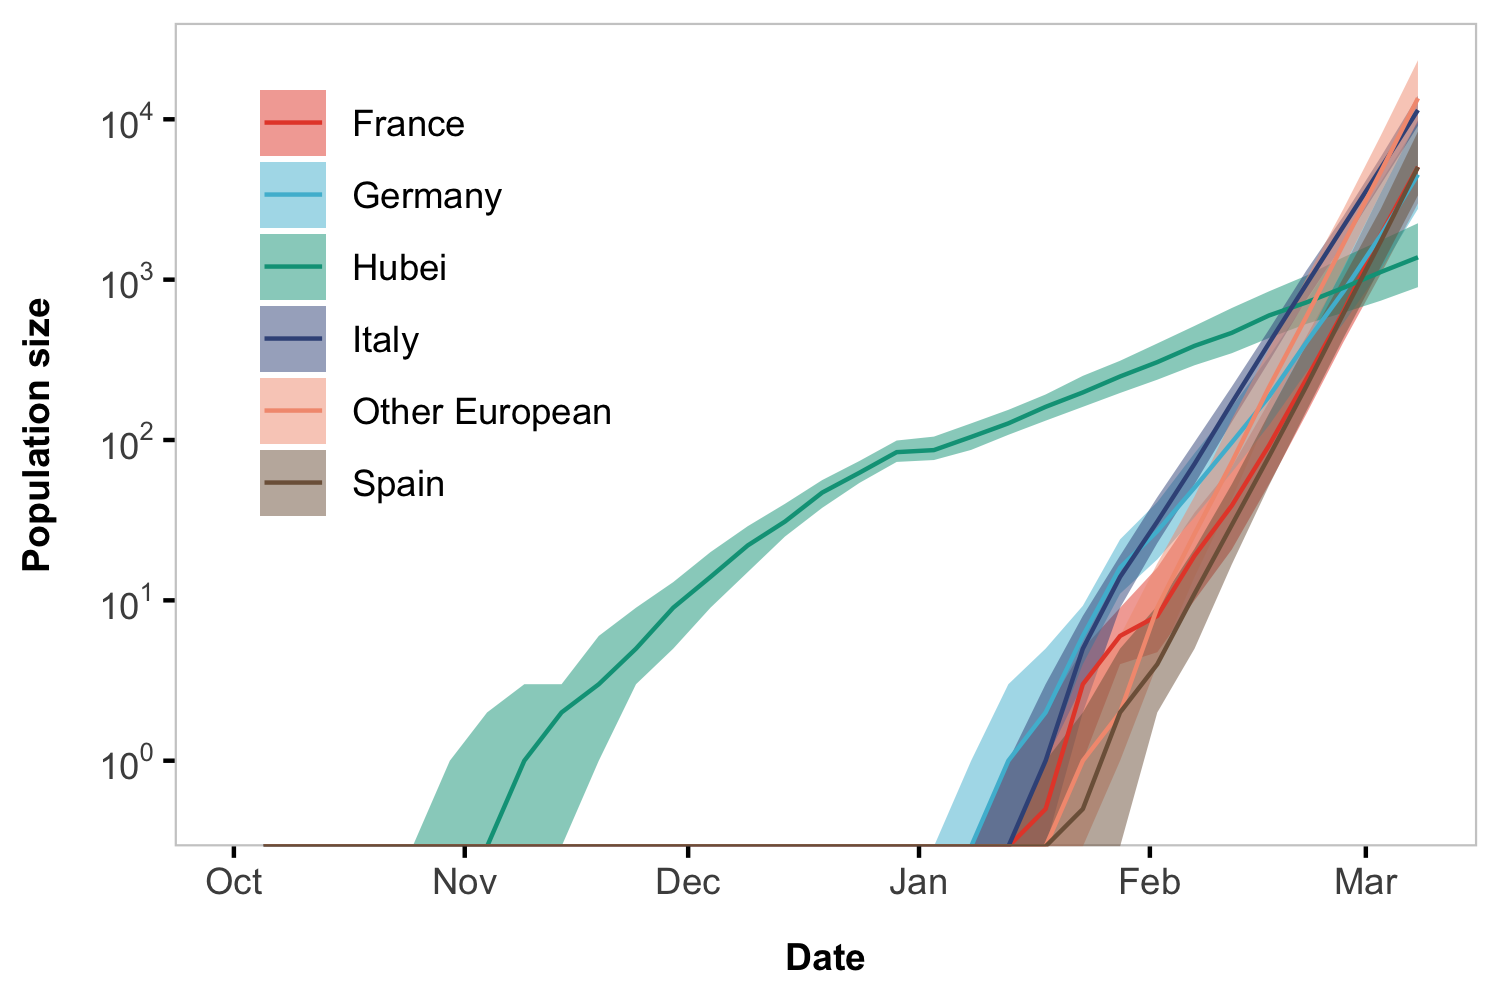
\includegraphics[width=0.8\textwidth]{201014_europe2_figtraj01.png}
    \caption{Inferred population size summary statistics for each deme over time. The line represents the median population trajectory and the interval is the interquartile range from a subsampled set of inferred population trajectories.}
    \label{fig:gribbon}
\end{figure}

\begin{figure}[h!]
    \centering
    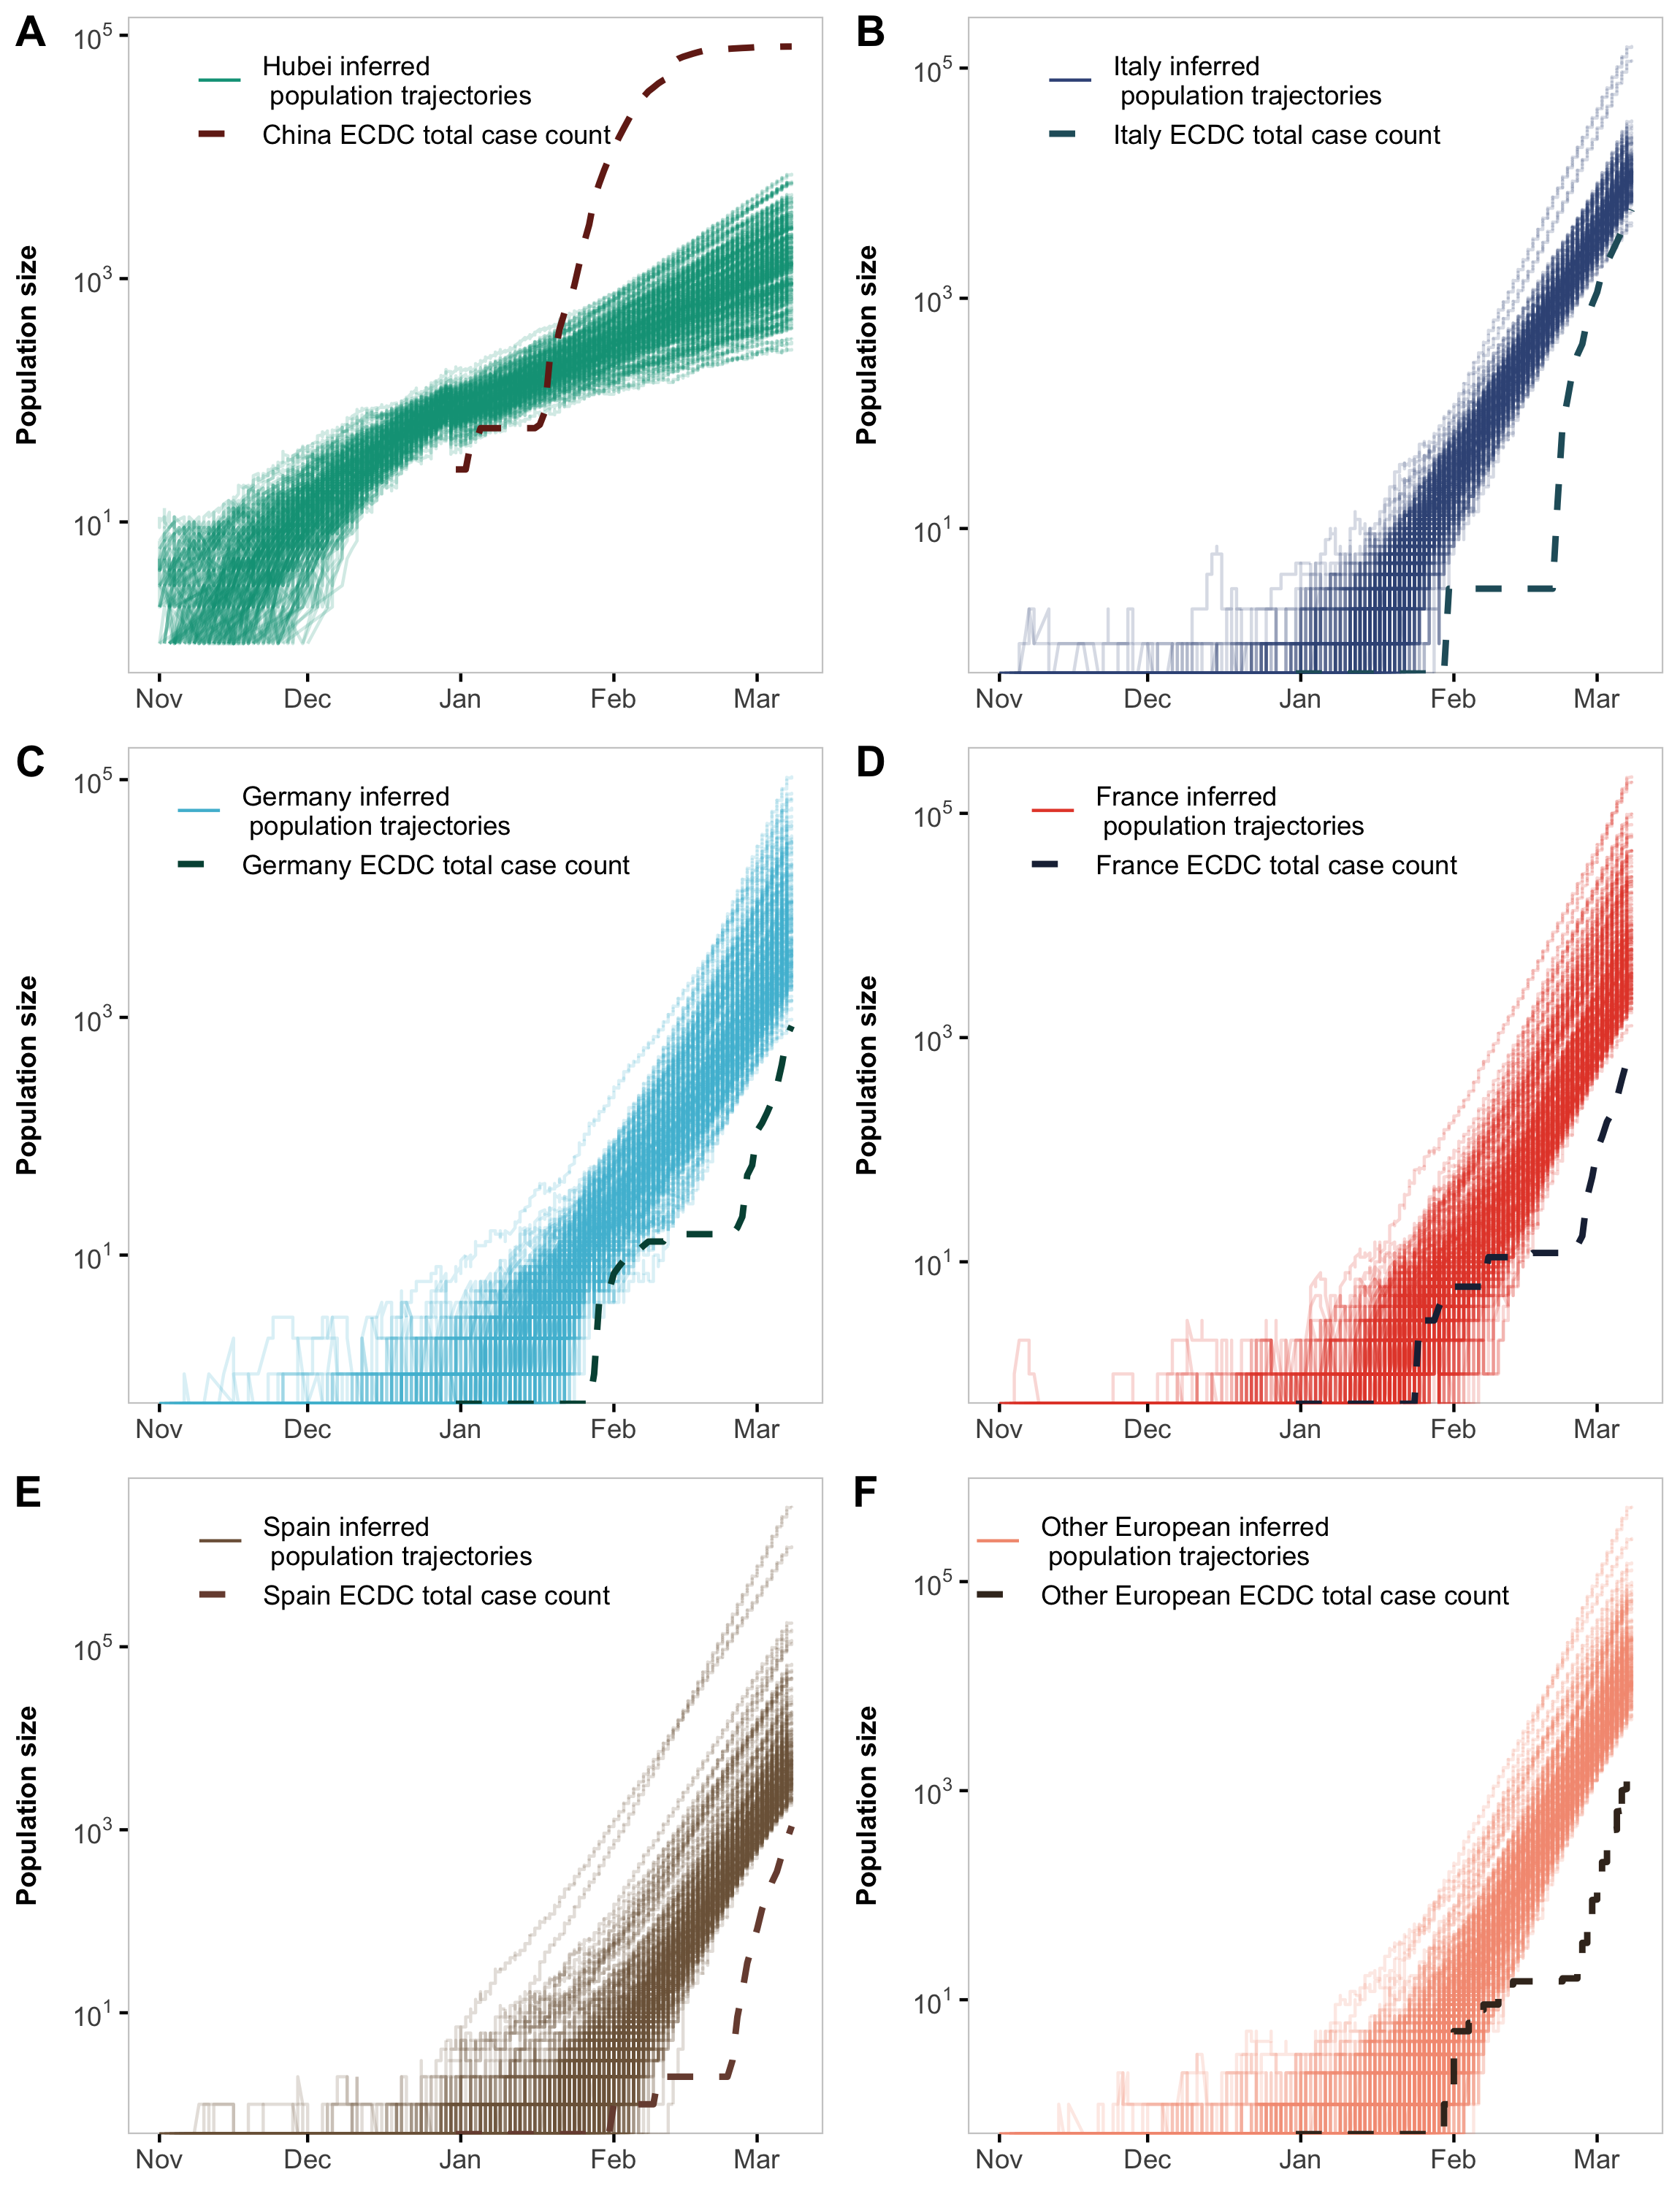
\includegraphics[width=0.9\textwidth]{201014_europe2_figtraj02.png}
    \caption{Inferred population size trajectories over time. A subsampled set of 200 inferred trajectories is plotted. In each subplot, the trajectories (solid lines) are compared with the ECDC total case count data (dashed line).}
    \label{fig:trajs}
\end{figure}


\begin{figure}[ht]
    \centering
    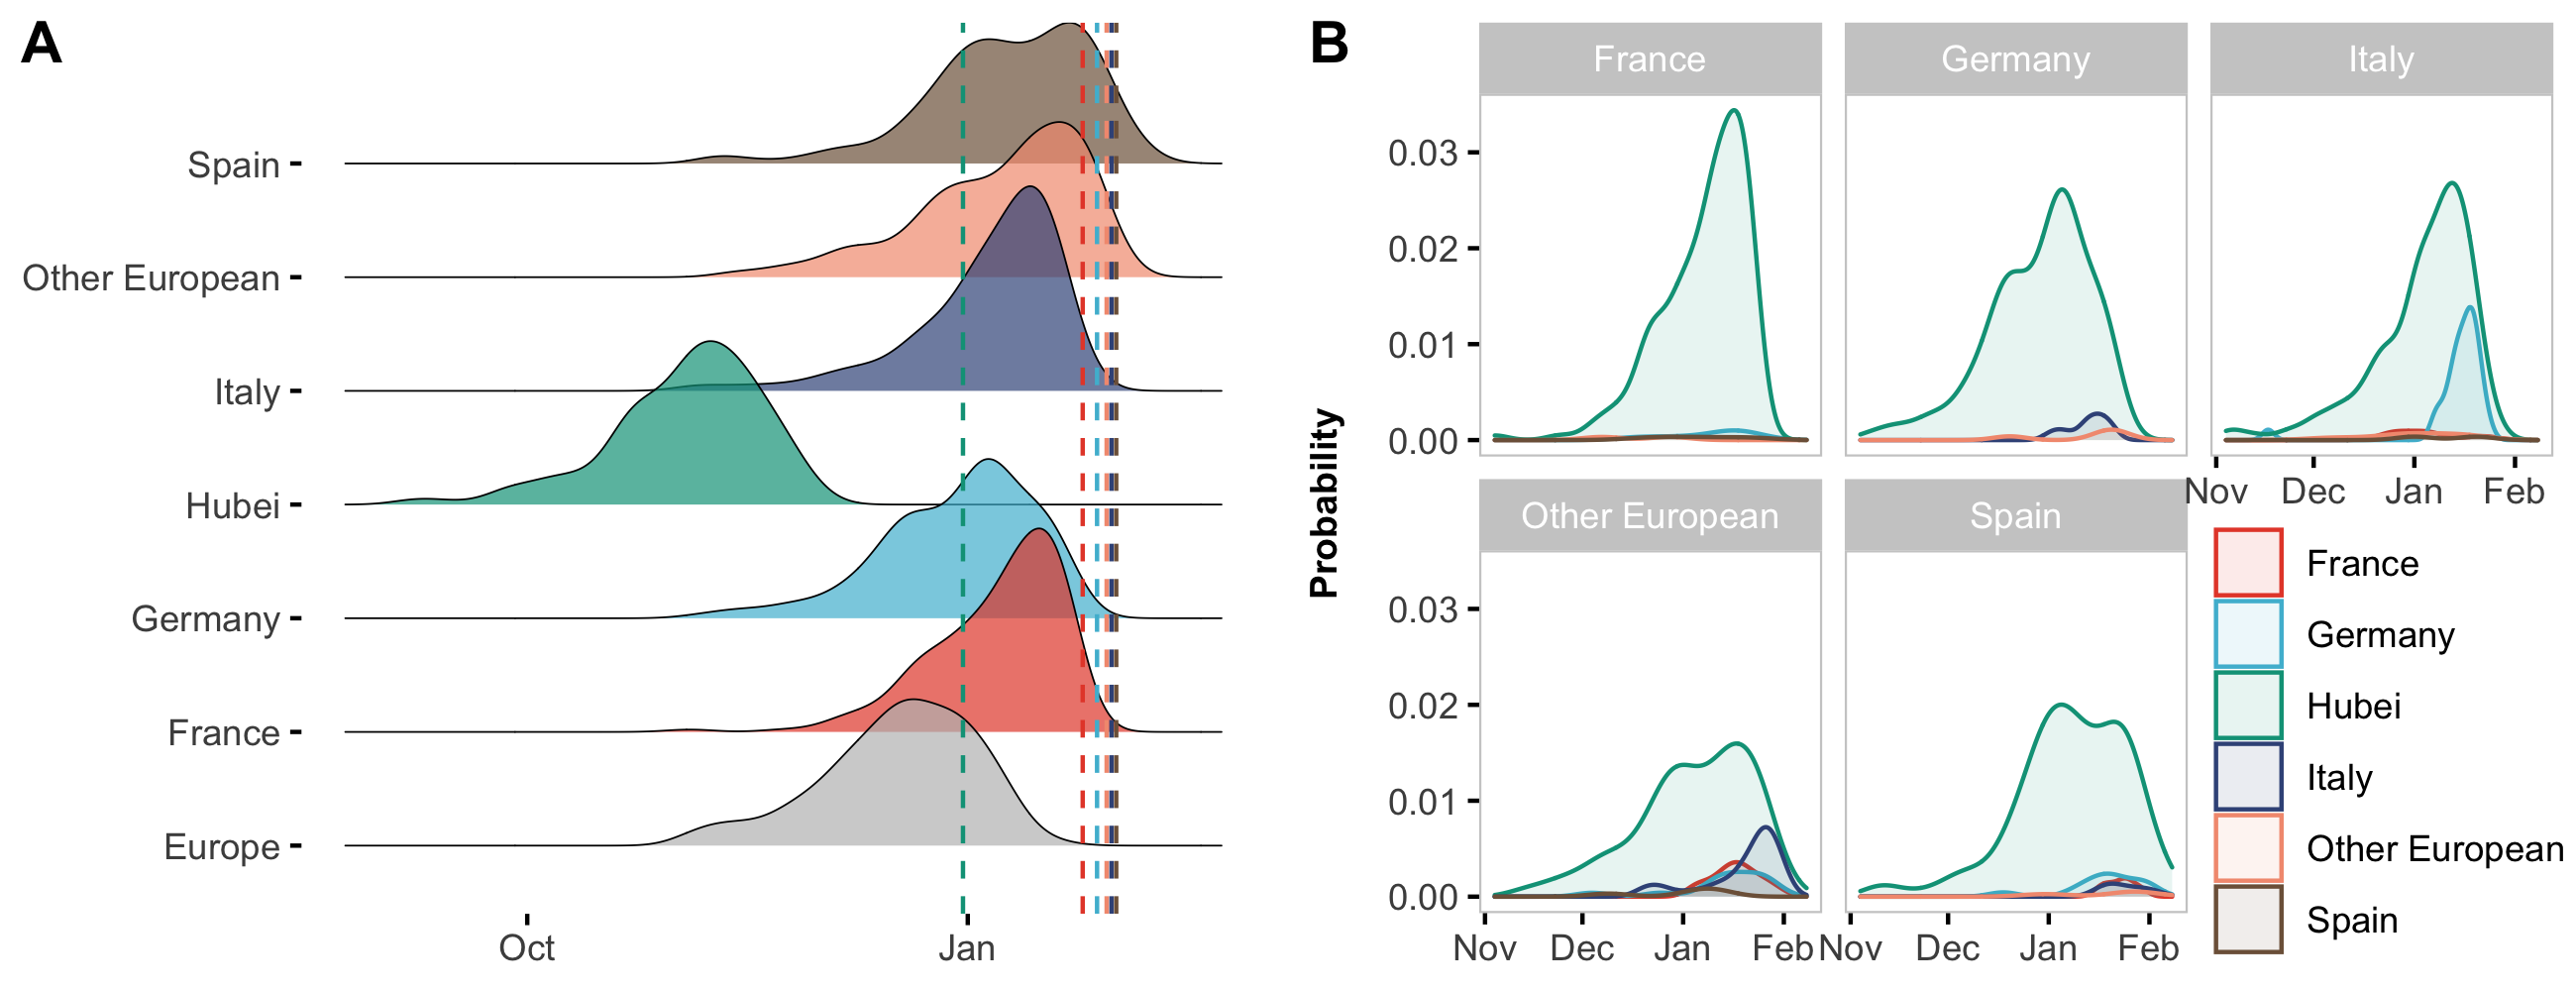
\includegraphics[width=\textwidth]{201014_europe2_figtraj03.png}
    \caption{First introductions event time and source in each deme. \textbf{A} Probability density of the time of the first introduction for each deme from the subsampled set of trajectories. Each dotted line represents the first date when cases where reported to ECDC by deme color. In the case of Hubei, the distribution of the time of the origin is plotted, since it was defined as the origin of the epidemic in the analysis with probability 1. For the other five demes, the distribution of the time of the first migration into the corresponding deme is plotted. \textbf{B} Probability density of the source of the first introduction event in each deme for the set of subsampled trajectories.}
    \label{fig:first}
\end{figure}

\begin{figure}[ht]
    \centering
    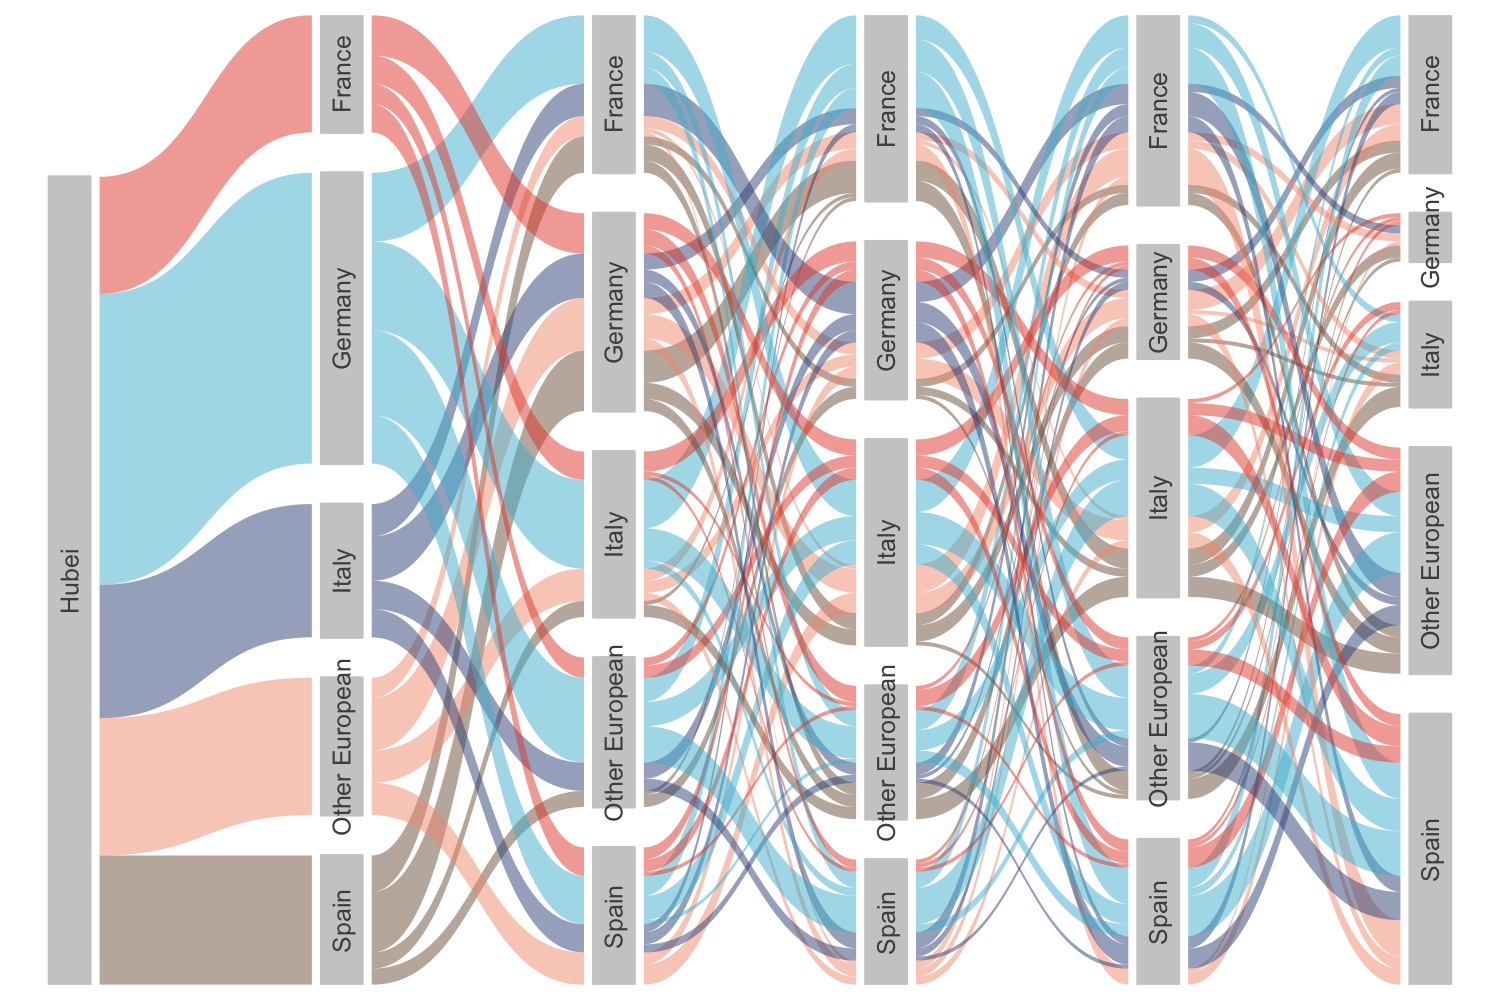
\includegraphics[width=\textwidth]{201014_europe2_figtraj04.png}
    \caption{}
    \label{fig:first_dest}
\end{figure}

\begin{figure}[ht]
    \centering
    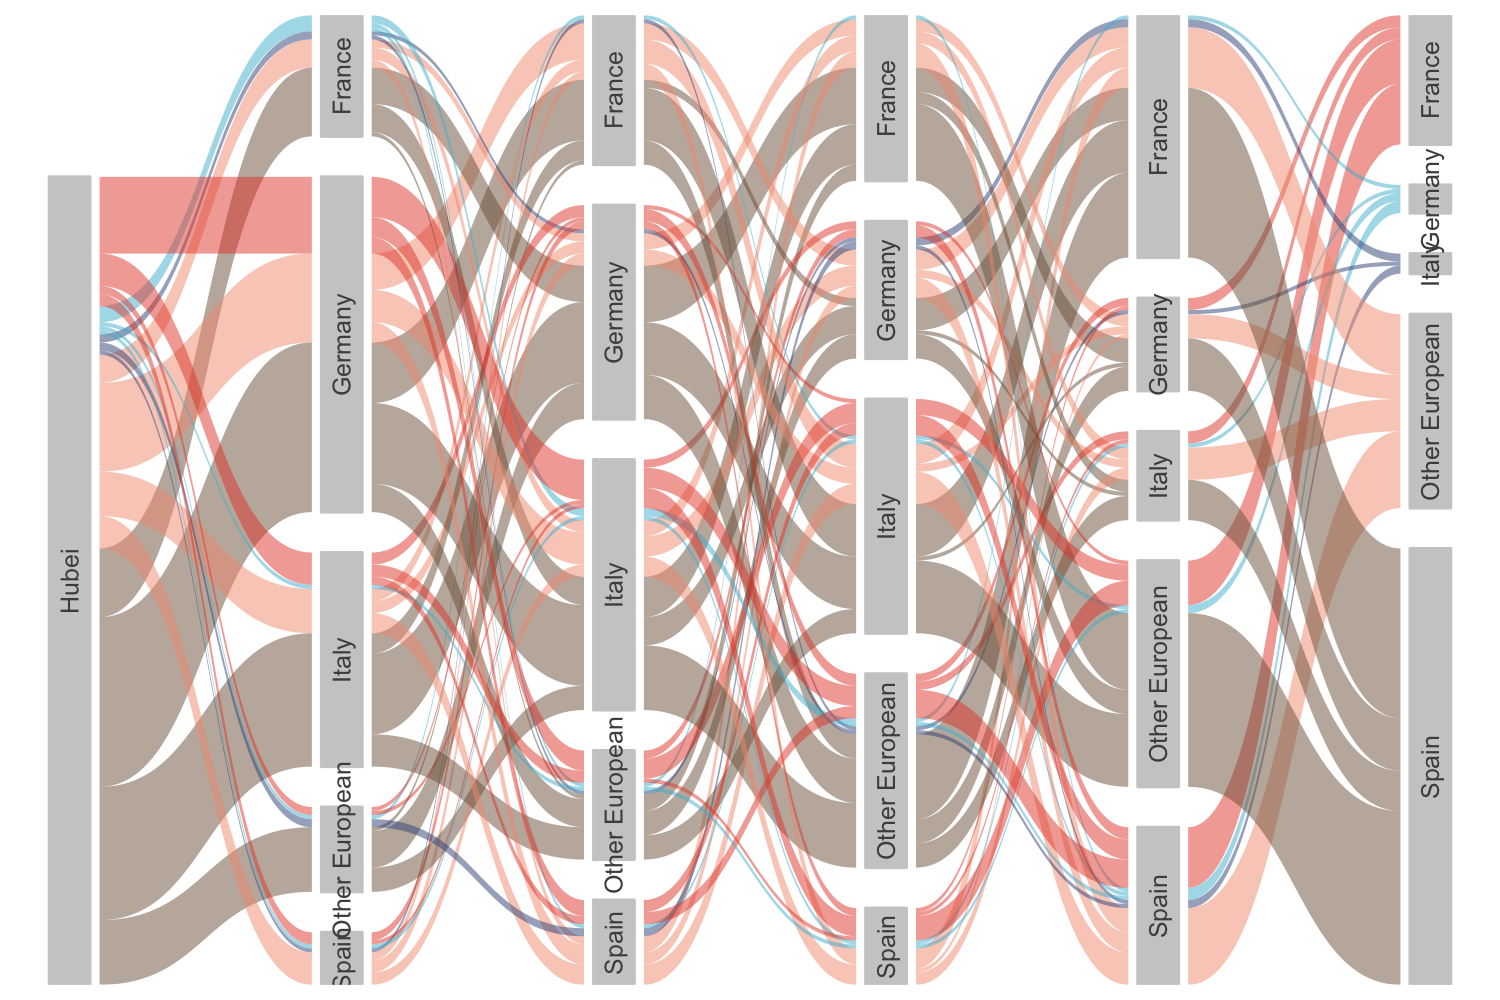
\includegraphics[width=\textwidth]{201014_europe2_figtraj05.png}
    \caption{}
    \label{fig:first_src}
\end{figure}

\begin{figure}[ht]
    \centering
    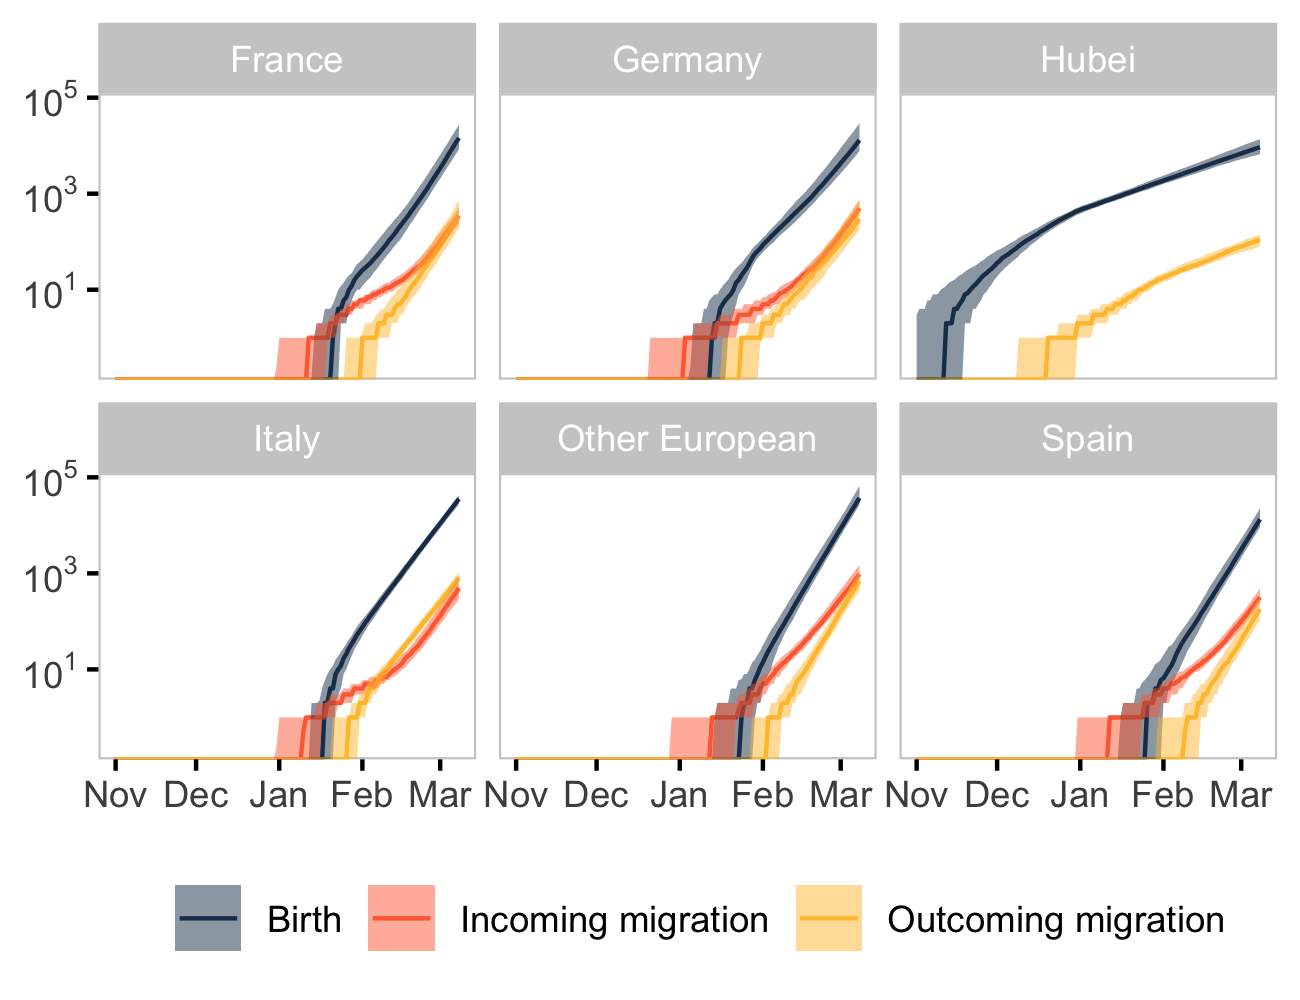
\includegraphics[width=\textwidth]{201014_europe2_figtraj06.png}
    \caption{Mean inferred cumulative number of events (births and migrations) over time. A subsampled set of 200 inferred trajectories is plotted.}
    \label{fig:events}
\end{figure}

\begin{figure}[ht]
    \centering
    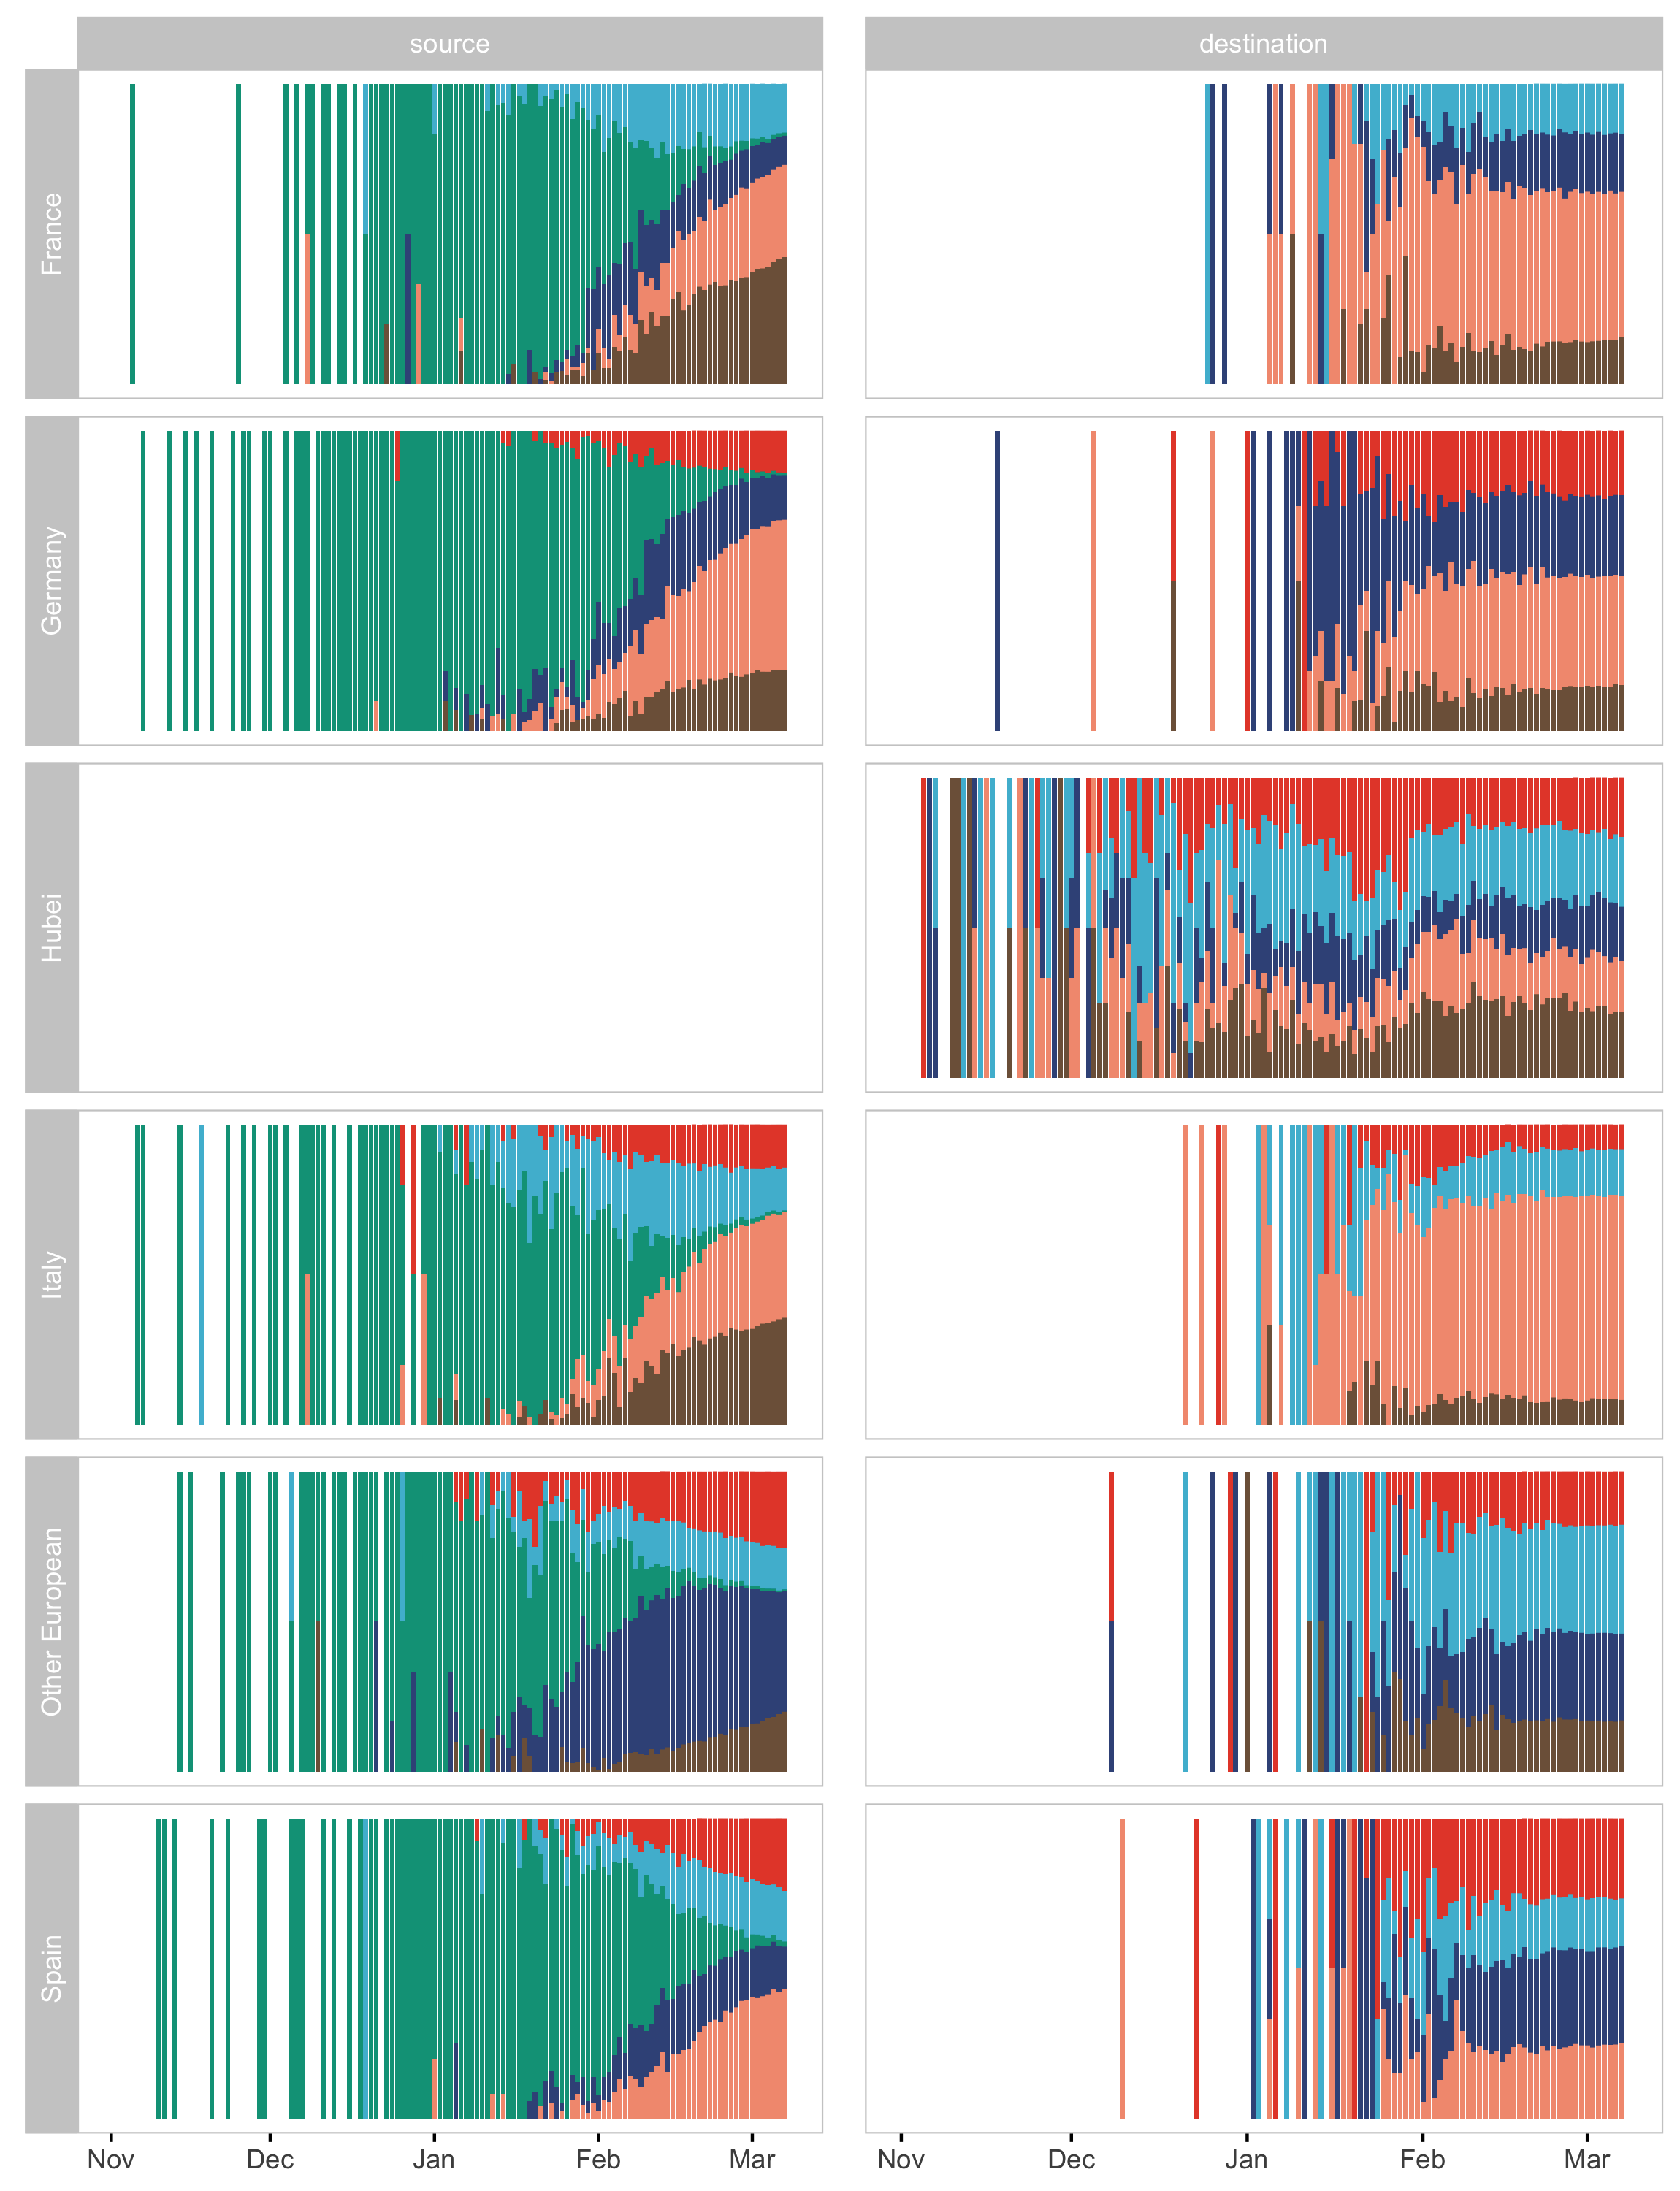
\includegraphics[width=\textwidth]{201014_europe2_figtraj07.png}
    \caption{}
    \label{fig:migs_srcdest}
\end{figure}


\begin{figure}[!tbp]
  \centering

  \begin{minipage}[t]{0.4\textwidth}
  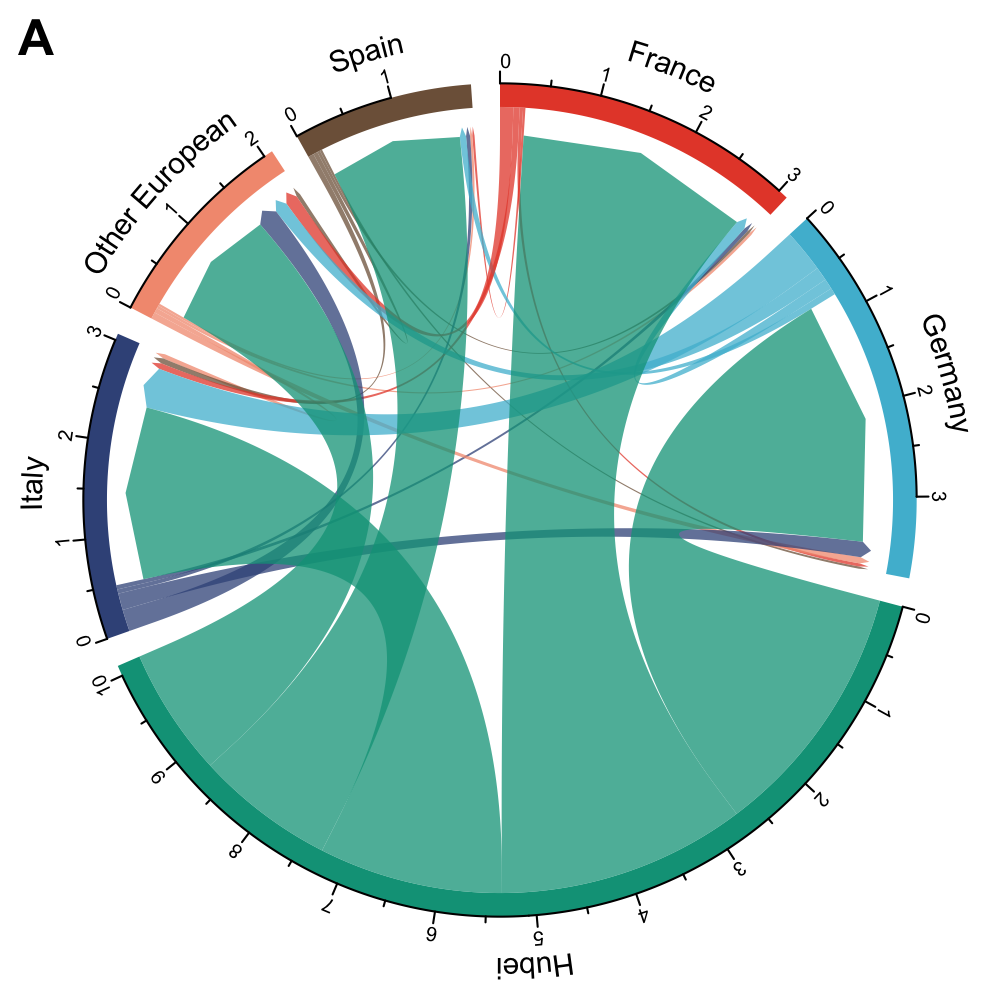
\includegraphics[width=\textwidth]{201014_europe2_figtraj08a.png}
  \label{fig:migs1}
  \end{minipage}
  \begin{minipage}[t]{0.4\textwidth}
  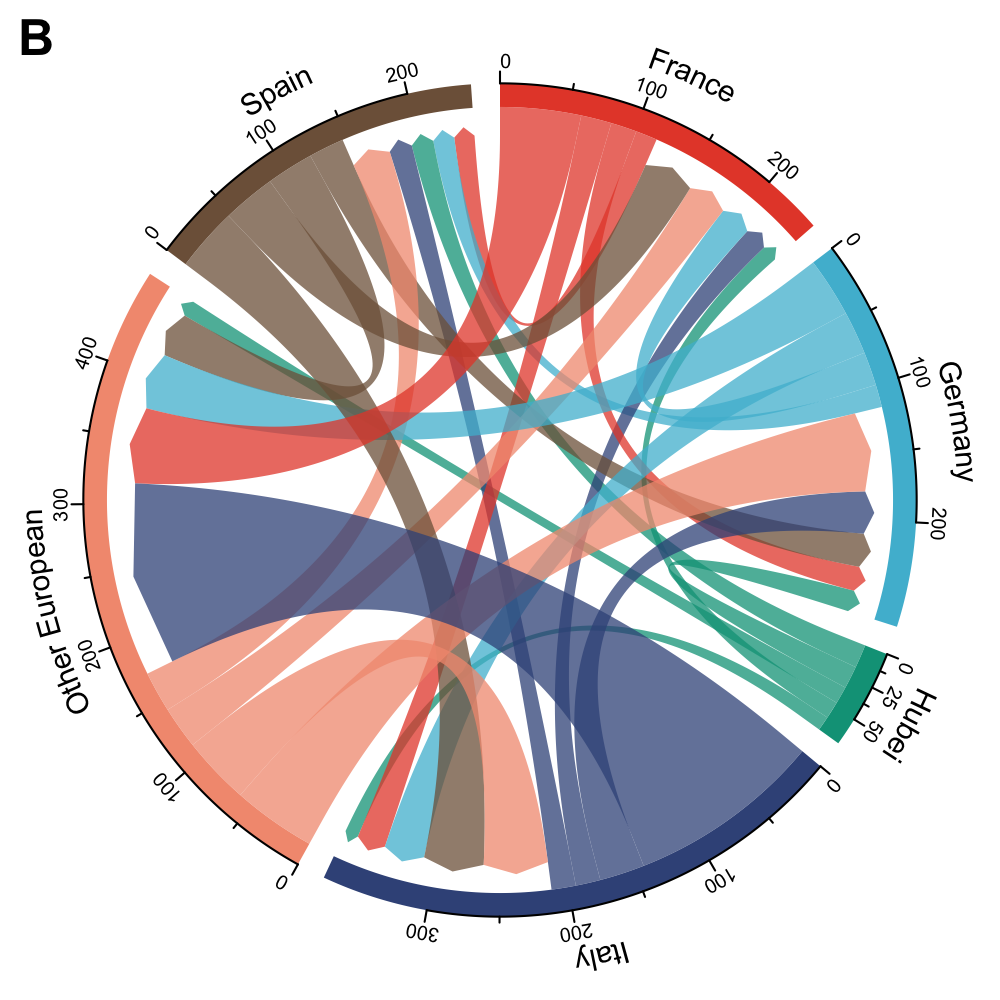
\includegraphics[width=\textwidth]{201014_europe2_figtraj08b.png}
  \label{fig:migs2}
  \end{minipage}
  \begin{minipage}[t]{0.4\textwidth}
  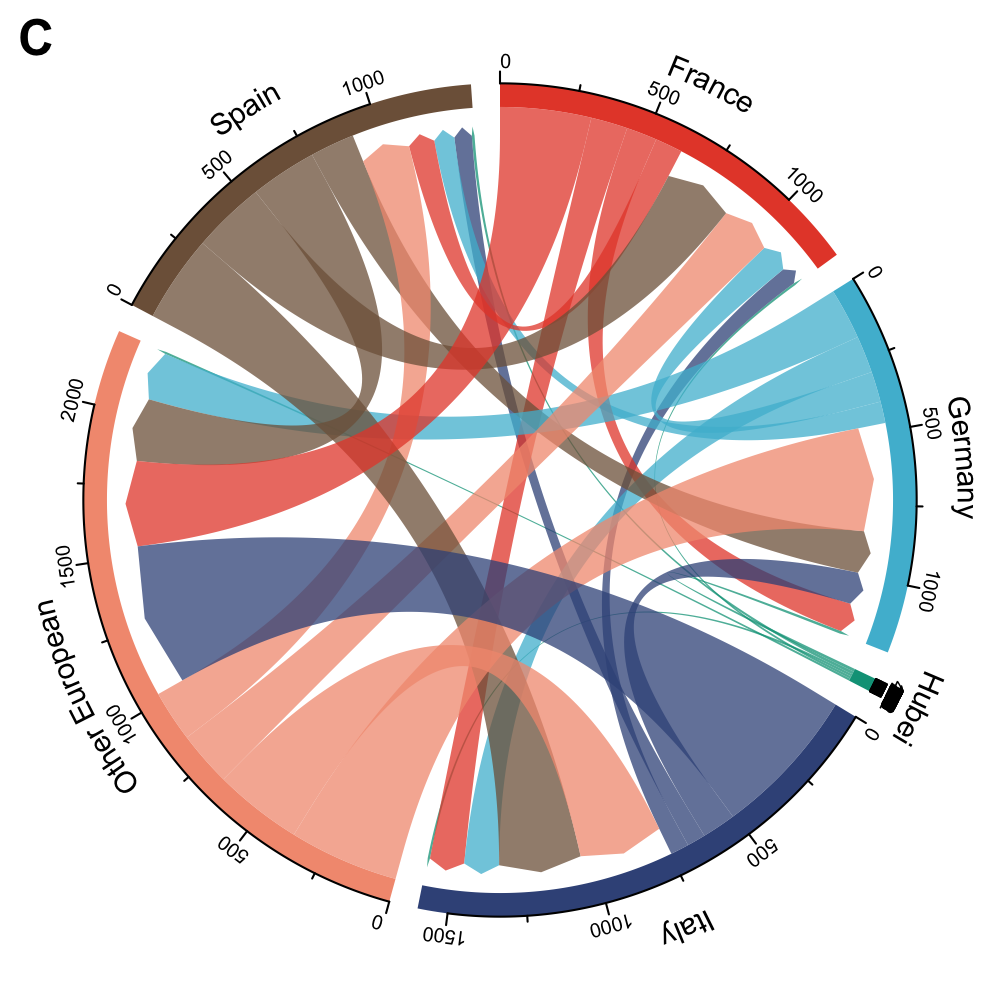
\includegraphics[width=\textwidth]{201014_europe2_figtraj08c.png}
  \label{fig:migs3}
  \end{minipage}
  \caption{Migration flux among demes over the three periods defined in the analysis.}
  \label{fig:migs}
\end{figure}

\end{document}